\section{图论与网络优化}
\subsection{图论的发展历史}
\subsubsection{七桥问题}
欧拉(图论之父)。\par
\xymatrix{
B\ar@(dl,ul)@{-}[dd]\ar@(dr,ur)@{-}[dd] & \\
\\
A\ar@(dl,ul)@{-}[dd]\ar@(dr,ur)@{-}[dd] & & & C\ar@{-}[lll]\ar@{-}[llluu]\ar@{-}[llldd] \\
\\\
D
}
\subsubsection{中国邮递员问题}
邮递员每天从邮局出发,走遍该地区所有街道再返回邮局,问题是他应如何安排送信的路线可以使所走的总路程最短。
\subsubsection{四色问题}
NP-Hard.

\subsection{图的基本概念}
\subsubsection{图的定义}
图是一个三元图
$$
G=\{V(G),E(G),\Psi(G)\}
$$
\iffalse
\begin{example}
\xymatrix{
 & $v_2$ & \\
 $v_1$ & & $v_3$ \\
  & $v_4$ &
}
this
\end{example}
\fi
\begin{align*}
V(G)=\{v_1,v_2,v_3,v_4\} \\
E(G)=\{e_1,e_2,e_3,e_4,e_5,e_6,e_7\} \\
\begin{cases}
\Psi_G(e_1)=v_1v_2 \\
\Psi_G(e_2)=v_2v_3 \\
\cdots
\end{cases}
\end{align*}
\subsubsection{有向图与无向图}
无向图:连接的边没有标注方向。\par
有向图:连接的边标注了方向。
赋权图:图中两点不仅关联,而且还标上了数量关系
\subsubsection{阶与度}
阶:图中顶点的数目。\par
度:与顶点的关联的边数。
\subsubsection{完全图}
在无向图中,任意两个顶点都存在着一条边。 \par
在有向图中,任意两个顶点都至少存在方向相反的两条边。
\subsubsection{子图}
如果
\begin{align*}
V(H) \in V(G) \\
E(H) \in E(G)
\end{align*}
称$H$是$G$的子图。
\subsubsection{道路与回路}
\begin{align*}
G=\{V(G),E(G)\} \\
e_i\in E(G),\quad 1\leq i\leq k,\\
\Psi_G(e_i)=v_{i-1}v_i,\quad v_i\in V(G) \\
W=v_0e_1v_1e_2v_2\cdots e_kv_k
\end{align*}
称$W$为一条道路。如果起点与终点重合,则称为回路。各边相异的道路称为行迹。各顶点相异的道路称为轨道。起点与终点重合的轨道称为圈。\par
欧拉道路:经过图中的每条边一次(仅),行遍所有的顶点的道路。相应地有欧拉回路:\par
哈密顿道路:经过图中的所有顶点一次(仅),行遍所有的边的道路。相应地有哈密顿回路。

\subsubsection{图的矩阵表示}
关联矩阵
\begin{equation*}
M(G)\,=\,\left(
\begin{matrix}
m_{11} & m_{12} & \cdots \\
m_{21} & \cdots & \cdots \\
\vdots & \vdots & \vdots \\
\end{matrix}
\right)
\end{equation*}
其中$m_{ij}$表示$v_i$与$e_j$的关系。

邻接矩阵表示法
\begin{equation*}
A=(a_{ij})_{m\times n}\,=\,\left(
\begin{matrix}
m_{11} & m_{12} & \cdots \\
m_{21} & \cdots & \cdots \\
\vdots & \vdots & \vdots \\
\end{matrix}
\right)
\end{equation*}
其中$m_{ij}$表示$v_i$与$v_j$的关系,取值为0或1.

\subsection{基本模型}
\subsubsection{最短路径模型}
\begin{enumerate}[I]
\item 求图中某一点到其他店的最短路径。Dijkstra标记算法。
\item 任意两点之间的最短路径。Floyd算法。
\end{enumerate}
\subsubsection{中国邮递员问题}
又被称为寻找欧拉回路的问题。\par
从邮局出发,走遍邮区的所有道路至少一次,再回到邮局,怎么走最短。Fleury算法。
\subsubsection{旅行商}
TSP问题(Traveling Salesman Problem):一个旅行商人要拜访n个城市,他必须选择所要走的路径,路径的限制是每个城市只能拜访一次,而且最后要回到原来出发的城市。\par
又被称为寻找哈密顿圈的问题。\par
首先构造初始解,再使用改进算法进行改进。\par
构造算法:Christofides算法,对角线完全算法\par
改进算法:二次逐次修正法,Feiring矩阵逐次改进法。

\newpage
\section{灾情巡视路线}
\subsection{题目}
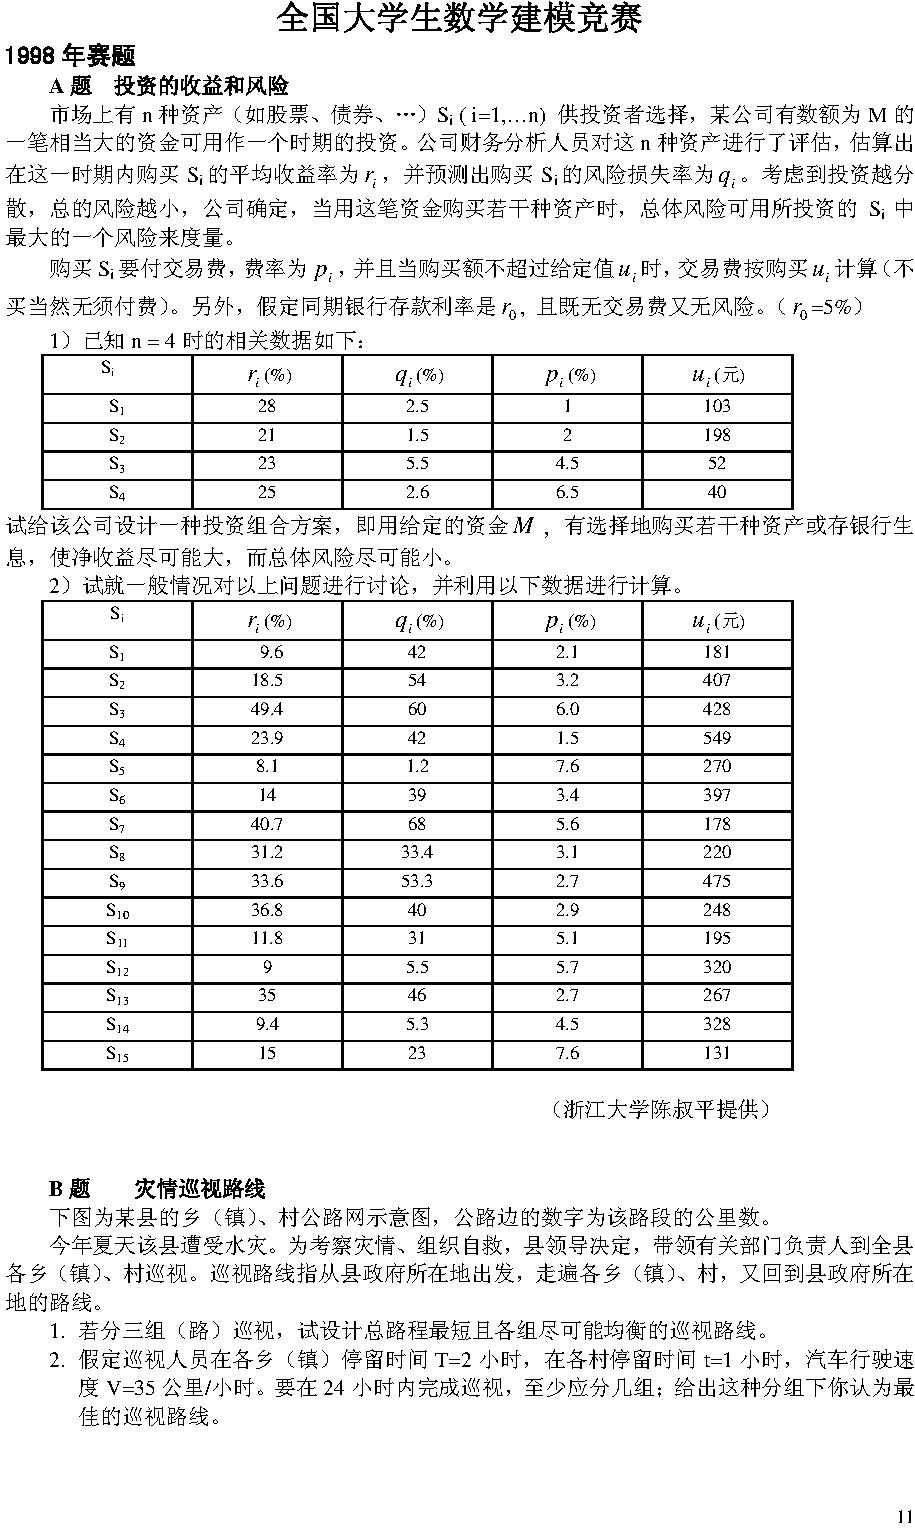
\includegraphics[width=0.9\textwidth,page=1]{Figures/1998}

\includegraphics[width=0.9\textwidth,page=2]{Figures/1998}

\subsection{模型的建立与分析}
把县、乡、村看作点,乡与村之间的公路看作边,距离看作对应边上的权。问题就转化为在加权有向图从给定点$O$出发,历经所有的顶点,使权值最短的问题。
算法(求图$G$的最佳经销商回路)
\begin{enumerate}
\item 用Dijkstra算法求出图G中任意两顶点之间的最短路,构造完备图$G'=(V,E')$。
\item 用对角线完全算法产生一个初始H圈。
\item 随机输入$G'$一个H圈。
\item 对第2、3、4步所得到的每个H圈,用改良圈法求一个近似最佳H圈。
\item 取第五步求出所有H圈中,权和最小者。
\end{enumerate}
\subsection{问题}
(1)若分三组(路)巡视,试设计总路程最短且各组尽可能均衡的巡视路线。
\begin{align*}
\text{顶点}O\in G(V_i),\quad i=1,2,\cdots,n. \\
\bigcup_{i=1}^nV_i\,=\,V(G), \\
\frac{\max_{i,j}\omega(C_i)-\omega(C_j)}{\max_i\omega(C_i)}\leq a, \\
\sum_{i=1}^n\omega(C_i)\,=\,\min
\end{align*}

(2)假定巡视人员在各乡(镇)停留时间 T=2 小时,在各村停留时间t=1 小时,汽车行驶速
度V=35 公里/小时。要在24 小时内完成巡视,至少应分几组;给出这种分组下你认为最
佳的巡视路线。\par
设分组数为n,$n>\frac{17*2+35}{24}$。通过计算发现当n=3时,时间啊方便不满足,所以采用n=4,具体路线需要通过计算得到。

(3)在上述关于 T , t 和V 的假定下,如果巡视人员足够多,完成巡视的最短时间是多少;给
出在这种最短时间完成巡视的要求下,你认为最佳的巡视路线。\par
\begin{enumerate}[(1)]
\item 每个巡视组总时间不超过6.43小时。
\item 所有点必须访问到,不得遗漏。
\item 巡视组要尽量少。
\end{enumerate}